\section{Evaluation}
\label{netqasm:sec:evaluation}
We evaluate two of the design choices that we made for \ac{NetQASM}:
    (1) exposing unit-modules to the \ac{CNPU} and
    (2) adding the possibility to use platform-specific flavors of instructions.
For both elements we study the difference in including them in \ac{NetQASM} versus not including them.
We do this by simulating a teleportation application and a blind quantum computation application.
These examples also showcase the ability of \ac{NetQASM} to express general quantum internet applications.

We have implemented a simulator, called SquidASM~\cite{git_squidasm}, that simulates a network in which end-nodes have the internal architecture as described in~\cref{sec:preliminaries}, that is, with an \ac{CNPU} and a \ac{QNPU}.
The simulator internally uses NetSquid~\cite{netsquid}, which was made specifically for the simulation of quantum networks.
SquidASM executes programs written using the SDK (\cref{sec:python-sdk}), including sending \ac{NetQASM} subroutines to the (simulated) \ac{QNPU}.
The code and data that were used to produce the results in this section can be found at~\cite{git_netqasm_paper_data}.

We evaluate the performance of \ac{NetQASM} by looking at the runtime quality of two applications, both consisting of two programs (one per node).
The first is a teleportation of a single qubit from a sender node to a receiver node.
We define the quality as the fidelity between the original qubit state at the sender and the final qubit state at the receiver.
The second application is a blind computation protocol which involves a client and a server.
The server effectively performs, blindly, a single-qubit computation on behalf of the client.
The protocol is a so-called \textit{verifiable blind quantum computation}~\cite{fitzsimons2017unconditionally}.
This means that some of the rounds of the protocols are \textit{trap rounds}.
We define the quality that we evaluate as the error rate of these trap rounds, since this indicates the blindness of the server.

We run these applications on SquidASM, where we simulate realistic quantum hardware.
Specifically, we simulate nodes based on nitrogen-vacancies (NV) in diamond, that can do heralded entanglement generation between each other.
The simulated hardware uses noise models that are also used in~\cite{coopmans2021netsquid}.
For more details, see~\cref{app:simulation}.

A note on how we chose what to evaluate and what not.
We listed several design considerations in ~\cref{sec:design_considerations}.
We addressed these in our design decisions (\cref{sec:design_decisions}).
For some of these, it is straightforward to see how they address a certain consideration, such as conditionals allowing for fast runtime feedback, and unit modules for allowing multitasking, as explained in~\cref{sec:design_decisions}.
Also, fundamental requirements like remote-entanglement generation and shared memory have been addressed.
The remaining considerations, and our solutions, namely platform independence and memory virtualization using unit modules, are less trivial to evaluate just by looking at the design.
Therefore, we focus on the evaluation of these two design decisions.

In our evaluation, we focus specifically on the Nitrogen-Vacancy hardware for our nodes.
This has two reasons.
First, it is a promising hardware platform for quantum network nodes~\cite{Taminiau2014} which we know quite well since it is available in the lab, and we have even used \ac{NetQASM} in a simple test case running on nodes based on NV~\cite{pompili2021experimental}.
Second, the NV hardware is interesting since it has a restricted gate set and qubit topology, which is explained in more detail below.
Therefore, we expect that the use of unit modules and an NV-specific flavor makes a difference in terms of runtime quality.

\subsection{Unit modules}
\label{netqasm:sec:evaluation-unit-modules}
We ask ourselves the question whether it pays off to expose unit modules, that is, a qubit topology with gate- and entanglement information.
Specifically, we want to know if there are situations where knowing the unit module gives the \ac{CNPU} an opportunity to optimize the application in a way that is not possible when not knowing the unit module.
If so, we are interested in how much advantage this gives (in terms of the runtime quality defined above).

In the next section we show that there are indeed situations where knowledge of the unit module is advantageous.
It can be that the order in which \ac{NetQASM} instructions are issued in a subroutine is sub-optimal, since virtual qubit IDs may be mapped in such a way that the \ac{QNPU} has to move virtual qubits to different physical qubits in order to execute the instructions.
If the \ac{CNPU} layer does not know this mapping, it cannot know that the instructions are ordered sub-optimally.
With knowledge of the unit module, on the other hand, the \ac{CNPU} can optimize the order and the overall application performance is improved.

We consider a teleportation application where a \textit{sender} program teleports a single qubit to another \textit{receiver} program.
It is assumed that the underlying platform is based on nitrogen-vacancy centers in diamond (NV) and use well-established models for both the noise and operations supported on such platforms, see \cref{app:simulation}.
The sender program uses two qubits: one to create entanglement with the receiver (qubit E), and one to send (teleport) to the receiver (qubit T).
At some point, the sender measures both qubits, after which it sends the outcomes to the receiver so that it can do the relevant corrections on its received qubit.
We assume that the sender program is written in a higher-level language like, like in our SDK (\cref{sec:sdk}), and in such a way that it first issues a measurement operation on qubit T, and then on E. However, due to the differences in characteristics of the physical qubits, as will be explained below, it is more efficient to first do the measurement on E, and then on T. Now we consider two scenarios, namely
\begin{itemize}
  \item \textbf{Unit-modules (UM)}.
        We assume that the sender program is written and executed on a software stack implementing \ac{NetQASM}, which means that the application's view of its quantum working memory is in the form of a unit module.
        This unit module contains information about the above-mentioned hardware restrictions, and therefore a compiler can take advantage of it by re-ordering the measurement operations while generating the \ac{NetQASM} subroutines to be sent to the \ac{QNPU}.
  \item \textbf{No unit-modules (NUM)}.
        In this case the software stack also implements \ac{NetQASM}, but without unit modules.
        Specifically, the application sees its quantum memory as just a number of uniform qubits.
        Therefore, a compiler for this application does not know about the hardware restrictions, and will construct \ac{NetQASM}-subroutines sent to the \ac{QNPU} without doing any optimization and leaves the order of the operations to be performed as they are specified in the high-level SDK.
\end{itemize}

Let's first go through the steps of the teleportation application:\newline
\begin{description}
  \item[\textit{sender}]:
        \begin{enumerate}
          \item Initialize qubit $q_t$ to be teleported in a Pauli state.
          \item Create entanglement with \textit{receiver} using qubit $q_s$.
          \item Perform CNOT gate with $q_t$ as control and $q_s$ as target.
          \item Perform Hadamard gate on $q_t$.
          \item Measure qubit $q_t$ and store outcome as $m_1$.
          \item Measure qubit $q_s$ and store outcome as $m_2$.
          \item Send $m_1$ and $m_2$ to \textit{receiver}.
        \end{enumerate}
  \item[\textit{receiver}]:
        \begin{enumerate}
          \item Receive entanglement with \textit{sender} using qubit $q_r$.
          \item Receive measurement outcomes from \textit{sender}.
          \item Apply correction operations on $q_r$ based on measurement outcomes.
        \end{enumerate}
\end{description}

We will now consider the order of the steps of the \textit{sender}.
Firstly, we assume that the qubit to be teleported, $q_t$, is always created before the entanglement.
We motivate this assumption below. For this reason, steps 1--3 and 7 are fixed and cannot change.
However, we are free to do step 6 before step 4 and 5, since these single-qubit operations and measurements commute, as long as we are consistent with the outcomes $m_1$ and $m_2$.
Let's now consider what impact this decision of measuring $q_s$ before $q_t$ or not has on the quality of execution for a NV-platform.

One of the biggest restrictions on a NV-platform is the topology of the qubits.
In particular, the NV-platform has a single communication-qubit (electron) surrounded by some number of storage qubits (carbon spins), see for example \cref{fig:topology}.
The single communication qubit is not only responsible for any remote entanglement generation but also for any two-qubit gate and is the only qubit that can be directly measured.
These restrictions require qubit states to be moved back and forth between the communication qubit and the storage qubits in order to free up the communication qubit, to create new entanglement or to measure another qubit.
Since the operation of moving a qubit state is relatively slow on this platform (up to a millisecond~\cite{Humphreys2018}) and adds noise to the qubits, it is important to try to minimize the number of moves needed.
For more details on the NV-platform, see for example~\cite{Bernien2014} or~\cite{dahlberg2019linklayer}.

In the steps of the \textit{sender} above, the communication qubit is first initialized to a Pauli state.
This state is then moved to a storage qubit to free up the communication qubit in order to create entanglement with the \textit{receiver}.
Then in step 5, $q_t$ should be measured, which is currently in the storage qubit.
This requires the qubit state to first be moved to the communication qubit.
However, at this point the communication qubit is occupied by the entangled pair and therefore first needs to be moved to a second storage qubit.
Qubit $q_t$ can then be moved to the communication qubit to be measured and then the same is done for $q_s$, requiring in total four move operations and three physical qubits.

We can now see that performing step 6 before 4 and 5 has the advantage that this qubit is already in the communication qubit and can be measured directly without moving it first.
Afterwards, $q_t$ can be moved to the communication qubit, which is cleared after the measurement, requiring in total only 2 move operations and only two physical qubits.
The decision of performing step 6 before 4 and 5 is highly dependent on the NV-platform and can only be made by a compiler that is aware about these restrictions.
The inclusion of unit-modules and qubit types in the \ac{NetQASM}-framework, which are exposed to the compiler at the \ac{CNPU}, allows for these optimization decision and can therefore improve the quality of execution.

For the two scenarios we consider, i.e. performing step 6 before 4 and 5 (\textbf{Unit modules (UM)}) or not (\textbf{No unit-modules (NUM)}), we check the average fidelity of the teleported state as a function of the gate noise (\cref{fig:sweep_gate_noise}), as well as the average fidelity and execution time as a function of gate duration (\cref{fig:sweep_gate_noise}), of the native two-qubit gate of the NV-platform. We see that performing step 6 before 4 and 5 improves both total execution time and average fidelity.
This can be explained by the fact that using unit modules allowed a compiler to produce \ac{NetQASM} code containing fewer two-qubit gates.
Therefore, an increase in two-qubit gate noise leads to a lower fidelity.
Also, an increase in two-qubit gate duration leads to higher execution time difference between the two scenarios.
Finally, \cref{fig:sweep_gate_noise} shows that the two-qubit gate duration does not affect the final fidelity in this situation, but the difference between using unit modules versus not using them remains.


\begin{figure}[t]
    \centering
    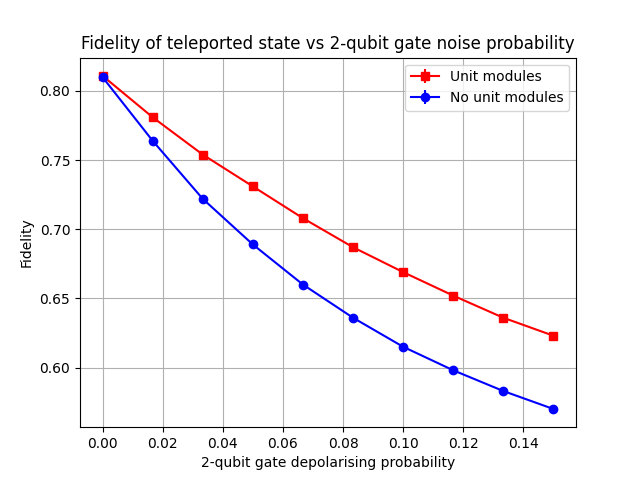
\includegraphics[scale=0.8]{figures/netqasm/plots/paper_teleport_sweep_gate_noise.png}
    \caption{
        Average fidelity between the original state at the sender and
        the final state at the server, as a function of the depolarizing noise
        of the native two-qubit gate of the NV-platform, both for the case of
        performing step 6 after (\textbf{No unit modules}) and before
        (\textbf{Unit modules}) step 4 and 5. Execution time of the native
        two-qubit gate is set to 0.5 ms. The rest of the parameters used are
        listed in \cref{app:simulation}. Each point is the average over each of
        the six Pauli states as initial state, repeated 100 times.}
    \label{fig:sweep_gate_noise}
\end{figure}

\begin{figure}[t]
    \centering
    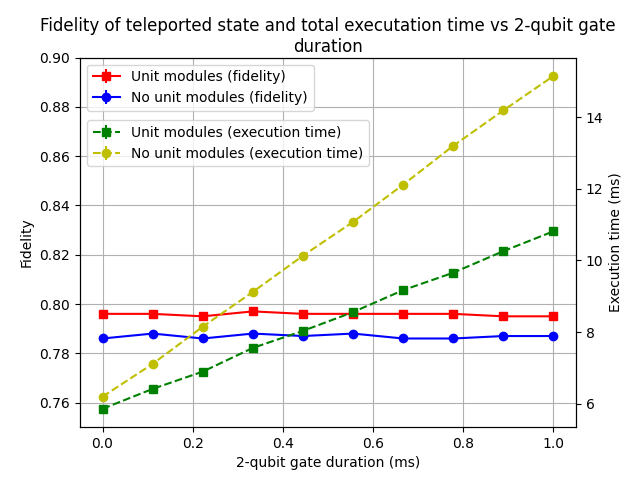
\includegraphics[scale=0.8]{figures/netqasm/plots/paper_teleport_sweep_gate_time.png}
    \caption{
        Average fidelity of the teleported state (left y-axis, solid lines) and total
        execution time of the teleportation application (right y-axis, dashed
        lines) as a function of the execution time of the native two-qubit gate
        of the NV-platform, both for the case of performing step 6 after
        (\textbf{No unit modules}) and before (\textbf{Unit modules}) step 4 and
        5. Dephasing parameter of the native two-qubit gate is set to 0.02. The
        rest of the parameters used are listed in \cref{app:simulation}. Each
        point is the average over each of the six Pauli state as initial state,
        repeated 100 times. In both figures, error bars are smaller than the drawn
        dots.}
  \label{fig:sweep_gate_time}
\end{figure}



\subsection{Flavors}
\label{netqasm:sec:evaluation-flavours}
While aiming to let \ac{NetQASM} be mostly platform-independent, we did also choose to allow platform-specific instructions, bundled in flavors.
The idea is that this allows for platform-specific optimization leading to better application performance.
Here we evaluate if flavors really impact potential performance, and if so how much.

We show that platform-specific optimization can indeed improve application performance, and that there are such optimizations that are not possible without flavors.
We see that it has impact mostly on the execution time, but not necessarily on outcome quality.

We consider the blind computation application depicted in \cref{fig:bqc_app}, where both the client and server node implement the NV hardware.
Again we compare two scenarios, in this case:
\begin{itemize}
  \item \textbf{Vanilla}.
        We compile both the client's and server's application code to \ac{NetQASM} subroutines with the vanilla flavor.
        The \ac{QNPU}, controlling NV hardware which does not implement all vanilla gates natively, needs to translate the vanilla instructions on the go.
        We assume this translation is ad-hoc and does not do any optimizations like removing redundant gates.
  \item \textbf{NV}.
        The code is compiled to \ac{NetQASM} subroutines containing instructions in the NV flavor, and redundant gates are optimized away.
        The \ac{QNPU} can directly execute the instructions on the hardware.
\end{itemize}

We implemented this by writing two separate programs in the SDK, one for the client and one for the server.
The SDK automatically compiles the relevant parts of these programs into \ac{NetQASM} subroutines.
Classical communication (values $\delta_1$, $m_1$ and $\delta_2)$ is done purely between the two simulated application layers, so these operations are not compiled to \ac{NetQASM} subroutines.
More details about the simulation can be found in \cref{app:simulation}.

The protocol is a verifiable blind quantum protocol~\cite{fitzsimons2017unconditionally}, which means that the circuit in~\cref{fig:bqc_app} is run multiple times, namely once per round.
Some of these rounds are \textit{trap rounds} in which the client chooses a special set of input values.
Such a trap round can either succeed or fail, depending on the values returned by the server.
The fraction of trap rounds that fail is called the error rate.
The error rate should stay low in order for the computation to be blind.

We simulate the BQC application by running the client's and server's programs in SquidASM.
We look at the error rate of the trap round as a function of the two-qubit gate noise.
The result can be seen in~\cref{fig:plot_bqc}.
It can be seen that using the NV flavor provides a better (lower) error rate than using the vanilla flavor.
This can be explained by noting that \ac{NetQASM} instructions in the vanilla flavor are mapped ad-hoc to native NV gates by the \ac{QNPU} at runtime, which leads to more two-qubit gates in total.


\begin{figure}[t]
  \centering
  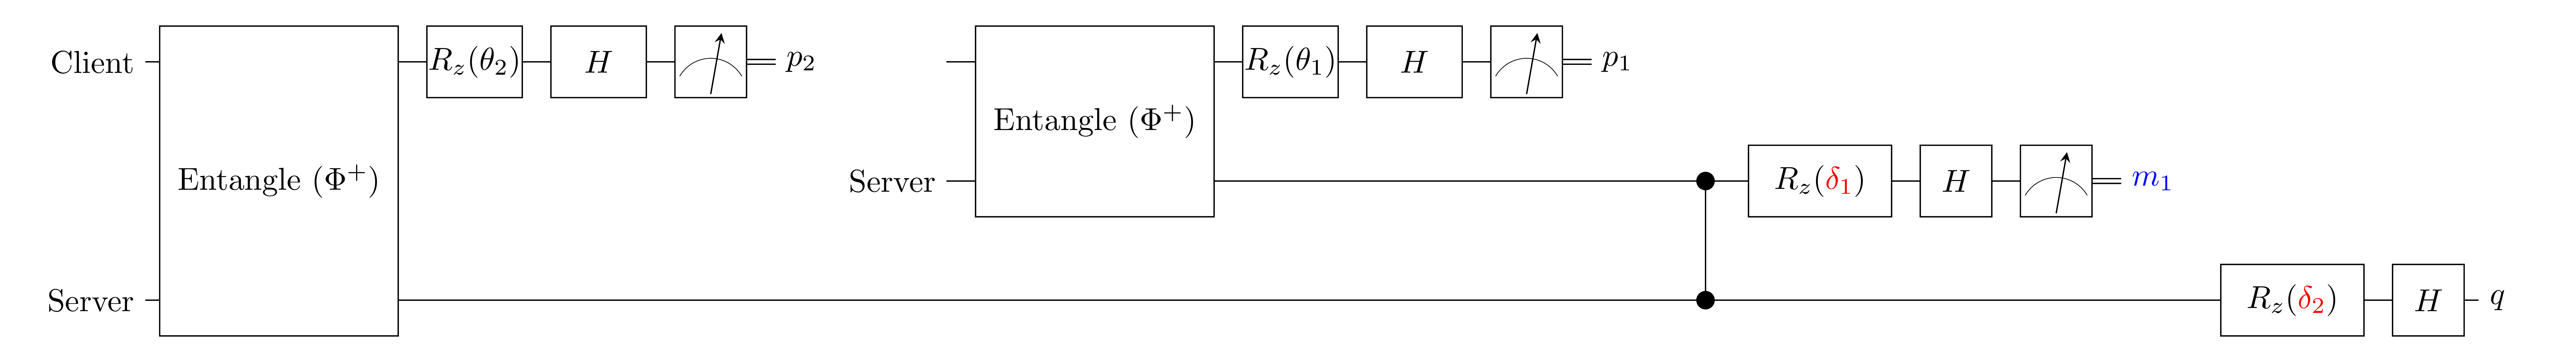
\includegraphics[width=0.6\linewidth]{figures/netqasm/bqc_app.png}
  \caption{Circuit representation of the simulated BQC application. The client
    remotely prepares two qubits on the server, by twice creating an
    entangled pair with the server followed by a local measurement. The
    server locally entangles its two qubits (cphase gate). Then, the client
    and server use classical communication to further guide the server's
    quantum operations. The client computes $\delta_1 = \alpha - \theta_1 +
      p_1 \cdot \pi$ and sends this to the server. The server uses the
    received value to do a local rotation and later sends measurement
    outcome $m_1$ back to the client. The client then sends $\delta_2 =
      (-1)^{m_1} \cdot (\beta - \theta_2 + p_2 \cdot \pi)$ to the server.
    The qubit state $q$ is the result of this application.
  }
  \label{fig:bqc_app}
\end{figure}


\begin{figure}[t]
  \centering
  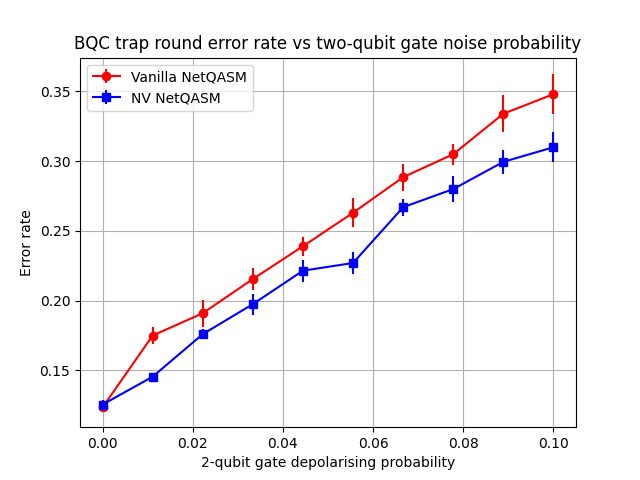
\includegraphics[scale=0.8]{figures/netqasm/plots/bqc_sweep_gate_noise_trap.png}
  \caption{
    Average error rate of trap rounds for the circuit of~\cref{fig:bqc_app}.
    Each point is the average over four combinations of $\theta_1$ and $\theta_2$,
    each used in 500 trap rounds. It can be seen that using the vanilla (platform-independent)
    \ac{NetQASM} flavor results in a worse (higher) error rate on average.}
  \label{fig:plot_bqc}
\end{figure}

To gain some more insight into why using the NV flavor provides a lower error rate we also look at the fidelity of the two quantum states on the server before any local gates are applied.
As can be seen in~\cref{fig:bqc_app}, the client remotely prepares two states on the server by twice creating entanglement and measuring its own half of the EPR pair.
In~\cref{fig:plot_bqc_fidelity} we see that already during this remote state preparation phase the NV flavor outperforms the vanilla flavor in terms of the fidelity of the prepared states.

\begin{figure}[t]
  \centering
  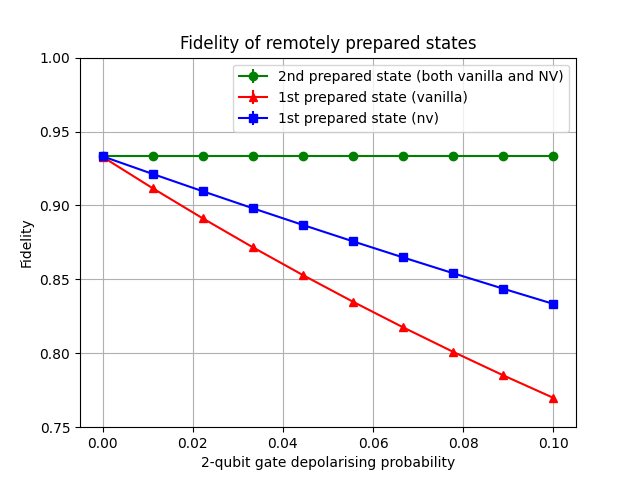
\includegraphics[scale=0.8]{figures/netqasm/plots/bqc_sweep_gate_noise_epr_fidelity.png}
  \caption{ Fidelity of the two remotely prepared states on the server in
        the BQC application. To remotely prepare a state, the client and server
        first create an EPR pair, and the client then measures its half in a
        specific basis while the server keeps its half stored in the
        communication qubit. This first prepared state is then moved to a memory
        qubit to free up the communication qubit for preparing the second state.
        This move operation has a negative effect on the fidelity of the first
        prepared state. Since the fidelity of the second prepared state only
        depends on the link entanglement generation, there is no difference
        between using vanilla or NV instructions. The values are from the same
        simulation experiment as for ~\cref{fig:plot_bqc}. Error bars are
        negligible.}
  \label{fig:plot_bqc_fidelity}
\end{figure}

\subsection{Relation to other results}
We note that a similar question of how many physical details to expose from lower-level layers (in our case the \ac{QNPU}) to higher-level layers (in our case the \ac{CNPU}) has also been evaluated in~\cite{murali2019fullstack}.
Their conclusion is that exposing and leveraging some of these details can indeed improve certain program success metrics.
That result agrees with that of ours, which shows that program execution quality can improve by exposing and leveraging unit modules and platform-specific \ac{NetQASM} flavors.

